\documentclass[conference]{IEEEtran}
\IEEEoverridecommandlockouts

\usepackage[T1]{fontenc}
\usepackage{cite}
\usepackage{amsmath,amssymb,amsfonts}
\usepackage{algorithmic}
\usepackage{graphicx}
\usepackage{textcomp}
\usepackage{booktabs}
\usepackage{array}
\usepackage{tikz}
\usepackage{pgfplots}
\pgfplotsset{compat=1.16}
\usetikzlibrary{positioning,arrows.meta,fit,backgrounds}
\usepackage[hidelinks]{hyperref}

\def\BibTeX{{\rm B\kern-.05em{\sc i\kern-.025em b}\kern-.08em
    T\kern-.1667em\lower.7ex\hbox{E}\kern-.125em X}}

\newcommand{\RMS}{\mathrm{RMS}}
\newcommand{\softmax}{\mathrm{softmax}}
\newcommand{\silu}{\mathrm{SiLU}}

\setlength{\textfloatsep}{5pt plus 2pt minus 2pt}
\setlength{\intextsep}{5pt}
\setlength{\abovedisplayskip}{2pt}\setlength{\belowdisplayskip}{2pt}
\setlength{\abovedisplayshortskip}{1pt}\setlength{\belowdisplayshortskip}{1pt}

\begin{document}

\title{Architecture Analysis of Qwen2.5-72B: A Dense, GQA-Based Decoder-Only Transformer with 128K Context}


\maketitle

\begin{abstract}
Qwen2.5-72B is the flagship open-weight dense model of Alibaba's Qwen2.5 family. This paper analyzes of its architecture, training methodology, and efficiency characteristics, based on the official technical report and related literature. The model is a decoder-only Transformer with 80 layers, a hidden size of 8192, Grouped-Query Attention (64 query / 8 key-value heads), SwiGLU feed-forward networks, rotary position embeddings, RMSNorm, and a byte-level BPE vocabulary of about 152K entries. It is pre-trained on 18 trillion tokens and extended to a 128K-token context at inference. We derive the parameter count (72.7B), KV-cache footprint and compute budget analytically and compare reported benchmarks with Llama-3/3.1 and Qwen2. The analysis shows that Qwen2.5-72B's gains over its predecessor stem mainly from data scale and quality and from post-training, rather than from structural changes to the Transformer block.
\end{abstract}

\begin{IEEEkeywords}
Qwen2.5, large language models, Transformer, grouped-query attention, SwiGLU, rotary embeddings, long context, inference efficiency
\end{IEEEkeywords}

%=====================================================================
\section{Introduction}
Qwen2.5 \cite{qwen25} comprises dense open-weight models from 0.5B to 72B parameters, plus two proprietary Mixture-of-Experts (MoE) variants. Its largest open model, Qwen2.5-72B, is reported to be competitive with Llama-3-405B while using roughly one-fifth of the parameters \cite{qwen25blog}. We study its architecture and mathematics (Sec.~II), training (Sec.~III), inference and compute (Sec.~IV), and benchmarks and comparisons (Sec.~V--VI). Quantities marked ``derived'' are our own analytical estimates from published hyper-parameters, not figures reported by the authors.

%=====================================================================
\section{Architecture}
\subsection{Overview and Specification}
Qwen2.5-72B retains the Qwen2 design \cite{qwen2}: a dense, decoder-only Transformer \cite{vaswani} built from pre-normalized blocks (Fig.~\ref{fig:arch}). Table~\ref{tab:spec} lists the specification. The model uses Grouped-Query Attention (GQA) \cite{gqa} for an efficient KV cache, SwiGLU activation \cite{glu}, rotary position embeddings (RoPE) \cite{rope}, RMSNorm \cite{rmsnorm} in a pre-norm arrangement, and a bias term on the QKV projections.

\begin{figure*}[t]
\centering
\resizebox{0.88\textwidth}{!}{%
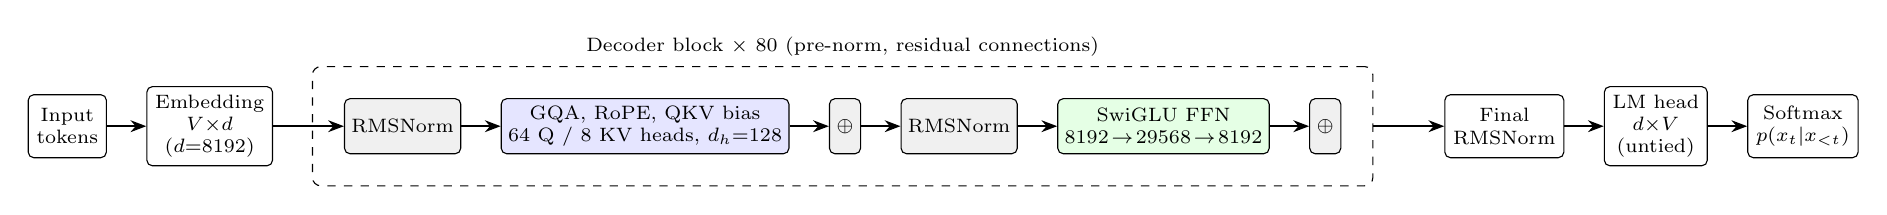
\begin{tikzpicture}[
  node distance=5mm,
  box/.style={draw,rounded corners=2pt,minimum height=8mm,align=center,font=\scriptsize,inner sep=3pt},
  sub/.style={draw,rounded corners=2pt,minimum height=7mm,align=center,font=\scriptsize,inner sep=2.5pt,fill=gray!12},
  ar/.style={-{Stealth[length=2mm]},thick}
]
\node[box] (tok) {Input\\tokens};
\node[box,right=of tok] (emb) {Embedding\\$V{\times}d$\\($d{=}8192$)};
\node[sub,right=9mm of emb] (n1) {RMSNorm};
\node[sub,right=of n1,fill=blue!10] (att) {GQA, RoPE, QKV bias\\64 Q / 8 KV heads, $d_h{=}128$};
\node[sub,right=of att] (add1) {$\oplus$};
\node[sub,right=of add1] (n2) {RMSNorm};
\node[sub,right=of n2,fill=green!10] (ffn) {SwiGLU FFN\\$8192\!\rightarrow\!29568\!\rightarrow\!8192$};
\node[sub,right=of ffn] (add2) {$\oplus$};
\begin{scope}[on background layer]
\node[draw,dashed,rounded corners=3pt,fit=(n1)(add2),inner sep=4mm,label={[font=\scriptsize]above:Decoder block $\times$ 80 (pre-norm, residual connections)}] (blk) {};
\end{scope}
\node[box,right=9mm of blk] (fn) {Final\\RMSNorm};
\node[box,right=of fn] (lm) {LM head\\$d{\times}V$\\(untied)};
\node[box,right=of lm] (out) {Softmax\\$p(x_t|x_{<t})$};
\draw[ar] (tok)--(emb); \draw[ar] (emb)--(n1);
\draw[ar] (n1)--(att); \draw[ar] (att)--(add1); \draw[ar] (add1)--(n2);
\draw[ar] (n2)--(ffn); \draw[ar] (ffn)--(add2); \draw[ar] (blk)--(fn);
\draw[ar] (fn)--(lm); \draw[ar] (lm)--(out);
\end{tikzpicture}}
\caption{Block diagram of Qwen2.5-72B (dense, decoder-only). Residual skip paths around each sub-layer are implied by the $\oplus$ nodes.}
\label{fig:arch}
\end{figure*}

\begin{table}[!tb]
\caption{Qwen2.5-72B Specification (from \cite{qwen25,qwen25blog}; * = derived)}
\label{tab:spec}
\centering\footnotesize
\begin{tabular}{@{}ll@{}}
\toprule
Parameter & Value \\
\midrule
Total / non-embedding params & 72.7B / 70.0B (reported) \\
Layers $L$ & 80 \\
Hidden size $d$ / FFN size $d_{ff}$ & 8192 / 29568 \\
Query / KV heads $H/G$ & 64 / 8 ($d_h{=}128$) \\
Context / generation length & 128K (131{,}072) / 8K \\
Vocabulary (byte-level BPE) & 151{,}643 regular tokens \\
Pre-training tokens & 18T \\
\bottomrule
\end{tabular}
\end{table}

\subsection{Attention Mechanism}
Let $X\in\mathbb{R}^{n\times d}$ be the normalized block input. With $H{=}64$ query heads and $G{=}8$ key/value heads, query head $h$ shares KV head $g(h)=\lfloor hG/H\rfloor$, i.e., eight query heads per KV group:
\begin{align}
Q_h &= XW^Q_h + b^Q_h,\quad K_g = XW^K_g + b^K_g,\quad V_g = XW^V_g + b^V_g,\\
A_h &= \softmax\!\Big(\tfrac{\mathcal{R}(Q_h)\,\mathcal{R}(K_{g(h)})^{\top}}{\sqrt{d_h}} + M\Big)V_{g(h)},\\
O &= \big[A_1\Vert\cdots\Vert A_H\big]W^O,
\end{align}
where $M$ is the causal mask and $\mathcal{R}$ applies RoPE. RoPE rotates each 2-D pair $(x_{2i},x_{2i+1})$ at position $m$ by angle $m\theta_i$, with $\theta_i=\beta^{-2i/d_h}$; the dot product then depends only on relative offsets \cite{rope}. The base $\beta$ is raised from $10^4$ to $10^6$ during long-context training using the adjusted-base-frequency (ABF) technique \cite{abf,qwen25}. GQA cuts KV projections and cache $8\times$ versus multi-head attention with little quality loss \cite{gqa}.

\subsection{Feed-Forward Network and Normalization}
Each FFN is a gated SwiGLU unit \cite{glu} with three matrices and an expansion ratio of $d_{ff}/d\approx 3.61$:
\begin{equation}
\mathrm{FFN}(x)=W_{\mathrm{down}}\big(\silu(W_{\mathrm{gate}}x)\odot W_{\mathrm{up}}x\big),
\end{equation}
with $\silu(z)=z\,\sigma(z)$. RMSNorm \cite{rmsnorm} omits mean-centering: $\mathrm{RMSNorm}(x)=\gamma\odot x/\RMS(x)$, $\RMS(x)=\sqrt{\tfrac1d\sum_i x_i^2+\epsilon}$. A block computes
\begin{equation}
x' = x+\mathrm{Attn}(\mathrm{RMSNorm}(x)),\qquad y = x'+\mathrm{FFN}(\mathrm{RMSNorm}(x')).
\end{equation}

\subsection{Tokenization}
Qwen2.5 uses byte-level BPE with 151,643 regular tokens; control tokens were expanded from 3 to 22 (e.g., for tool use) and the vocabulary is unified across model sizes \cite{qwen25}.

\subsection{Parameter Count (Derived)}
Per layer, attention holds $2d^2+2d\,(Gd_h)$ weights (Q, O and the narrower K, V) and the FFN holds $3d\,d_{ff}$:
\begin{equation}
P \approx \underbrace{2Vd}_{\text{untied embed/head}} + L\big[2d^2+2dGd_h+3d\,d_{ff}\big].
\end{equation}
With $d{=}8192$, $Gd_h{=}1024$, $d_{ff}{=}29568$: attention $\approx 151.0$M and FFN $\approx 726.7$M per layer, i.e., $\approx 70.2$B transformer weights; with $V\!\approx\!152$K the embedding and head add $\approx 2.5$B, giving $\approx 72.7$B, matching the reported total (the reported 70.0B non-embedding figure differs slightly, likely from counting conventions).

%=====================================================================
\section{Training Methodology}
\subsection{Pre-training}
Pre-training data grew from 7T tokens (Qwen2) to 18T tokens \cite{qwen25}. Reported data steps: (i) quality filtering with Qwen2-Instruct models as scorers; (ii) inclusion of Qwen2.5-Math/Coder corpora; (iii) synthetic data from Qwen2-72B-Instruct and Qwen2-Math-72B-Instruct, filtered by reward models; and (iv) mixture rebalancing that down-samples e-commerce and social-media text and up-samples technical and academic text. Training minimizes the next-token cross-entropy
\begin{equation}
\mathcal{L}(\theta)=-\frac{1}{T}\sum_{t=1}^{T}\log p_\theta(x_t\mid x_{<t}).
\end{equation}
Hyper-parameters (learning rate, batch size) were set by scaling laws fitted across model sizes and data volumes \cite{qwen25}. At 18T tokens the 72B model sees $\approx 250$ tokens per parameter, far beyond the $\approx 20$ tokens/parameter Chinchilla optimum \cite{chinchilla}, trading training compute for cheaper serving.

\subsection{Long-Context Training}
Training proceeds in two phases: 4,096-token sequences, then an extension to 32,768 tokens in which the RoPE base is increased to $10^6$ via ABF \cite{abf}. Inference-time YaRN \cite{yarn} and Dual Chunk Attention (DCA) \cite{dca} extend this to 128K tokens.

\subsection{Post-Training}
Supervised fine-tuning uses over 1M samples (long-sequence output up to 8K tokens, math, code, structured data, reasoning). Alignment then combines offline Direct Preference Optimization (DPO) \cite{dpo} with online Group Relative Policy Optimization (GRPO) \cite{grpo}. GRPO removes the value network by normalizing rewards within a group of $K$ sampled responses:
\begin{equation}
\hat{A}_i=\frac{r_i-\mathrm{mean}(\{r_j\}_{j=1}^K)}{\mathrm{std}(\{r_j\}_{j=1}^K)},
\end{equation}
which is used in a clipped policy-gradient objective with a KL penalty to a reference policy \cite{grpo}.

%=====================================================================
\section{Inference Efficiency and Computational Requirements}
\subsection{KV Cache}
GQA's principal benefit is cache size. With $B_p$ bytes per element, a sequence of $s$ tokens requires
\begin{equation}
M_{KV}=2\,L\,G\,d_h\,s\,B_p .
\end{equation}
For $L{=}80$, $G{=}8$, $d_h{=}128$, $B_p{=}2$ (bf16): 320\,KiB per token (derived), i.e., $\approx 40$\,GiB at $s{=}131{,}072$ per sequence. Multi-head attention ($G{=}64$) would need 2.5\,MiB per token ($\approx 320$\,GiB at 128K), which is infeasible on commodity nodes.

\subsection{Compute and Memory}
Forward compute per token is $\approx 2N_{\mathrm{nonemb}}\approx 1.4\times10^{11}$ FLOPs plus attention cost $\approx 4\,L\,d\,s$ FLOPs for context $s$ ($\approx 3.4\times10^{11}$ at $s{=}131{,}072$, so attention dominates at long context). Training cost follows $C\approx 6ND\approx 7.8\times10^{24}$ FLOPs for $N{=}72.7$B, $D{=}18$T (derived). Weights occupy $\approx 145$\,GB in bf16, needing at least two 80\,GB accelerators, or $\approx 36$--$40$\,GB at 4 bits with AWQ-style quantization \cite{awq}. Decoding is memory-bandwidth bound: batch-1 throughput is at most $\mathrm{BW}/\text{bytes}_{\mathrm{weights}}$, so batching raises utilization.

%=====================================================================
\section{Benchmark Performance}
Table~\ref{tab:base} gives base-model results reported in \cite{qwen25blog}. All numbers are vendor-reported and use the source's evaluation settings (e.g., MMLU 5-shot, GSM8K 4-shot, HumanEval 0-shot).

\begin{table}[!tb]
\caption{Base-Model Benchmarks (reported in \cite{qwen25blog})}
\label{tab:base}
\centering\footnotesize
\setlength{\tabcolsep}{3.2pt}
\begin{tabular}{@{}lcccc@{}}
\toprule
Benchmark & Llama-3 & Llama-3 & Qwen2 & Qwen2.5 \\
 & 70B & 405B & 72B & 72B \\
\midrule
MMLU & 79.5 & 85.2 & 84.2 & \textbf{86.1} \\
MMLU-Pro & 52.8 & \textbf{61.6} & 55.7 & 58.1 \\
BBH & 81.0 & 85.9 & 82.4 & \textbf{86.3} \\
GPQA & 36.3 & -- & 37.4 & \textbf{45.9} \\
GSM8K & 77.6 & 89.0 & 89.0 & \textbf{91.5} \\
MATH & 42.5 & 53.8 & 50.9 & \textbf{62.1} \\
HumanEval & 48.2 & \textbf{61.0} & 64.6 & 59.1 \\
MBPP & 70.4 & 73.0 & 76.9 & \textbf{84.7} \\
\bottomrule
\end{tabular}
\end{table}

Qwen2.5-72B improves on Qwen2-72B on most base benchmarks, most strongly on GPQA ($+8.5$), MATH ($+11.2$) and MBPP ($+7.8$), and matches or exceeds Llama-3-405B on several (MMLU, BBH, GSM8K, MATH, MBPP) at about one-fifth the parameters. Llama-3-405B remains ahead on MMLU-Pro and HumanEval, and Qwen2.5-72B is below Qwen2 on HumanEval. For the instruction-tuned model the source reports MATH 83.1 (Llama-3.1-405B: 73.8), MBPP 88.2 (84.5), LiveCodeBench 55.5 (41.6) and Arena-Hard 81.2 (69.3), while Llama-3.1-405B leads on MMLU-Pro (73.3 vs.\ 71.1) and IFEval (86.0 vs.\ 84.1).

%=====================================================================
\section{Comparison and Key Innovations}
Table~\ref{tab:arch} contrasts the architectures. Qwen2.5-72B shares the depth, width and GQA layout of Llama-3.1-70B \cite{llama3}, differing in a slightly wider FFN, a larger vocabulary and QKV bias; Llama-3.1-405B is deeper and wider ($5.6\times$ the parameters). Qwen2.5-72B is architecturally almost identical to Qwen2-72B \cite{qwen2}; the differences are data (7T$\rightarrow$18T tokens), composition, and post-training.

\begin{table}[!tb]
\caption{Architectural Comparison with Contemporary Dense LLMs}
\label{tab:arch}
\centering\footnotesize
\setlength{\tabcolsep}{2.5pt}
\begin{tabular}{@{}lcccc@{}}
\toprule
 & Qwen2.5 & Qwen2 & Llama-3.1 & Llama-3.1 \\
 & 72B & 72B & 70B & 405B \\
\midrule
Layers & 80 & 80 & 80 & 126 \\
Hidden $d$ & 8192 & 8192 & 8192 & 16384 \\
FFN $d_{ff}$ & 29568 & 29568 & 28672 & 53248 \\
Heads (Q/KV) & 64/8 & 64/8 & 64/8 & 128/8 \\
Vocab. & $\sim$152K & $\sim$152K & 128K & 128K \\
Train tokens & 18T & 7T & $\sim$15T & 15.6T \\
\bottomrule
\end{tabular}
\end{table}

The innovations are therefore mostly in \textit{process}: (1) 18T-token pre-training with model-based filtering and domain-specific synthetic data; (2) scaling-law-based hyper-parameter selection; (3) staged long-context training combined with training-free length extrapolation (YaRN, DCA); (4) a multi-stage alignment pipeline (SFT, DPO, GRPO); and (5) a unified vocabulary with expanded control tokens that eases tool use and cross-size compatibility. Caveats: training hardware, mixture proportions and optimizer settings are undisclosed, and benchmark numbers are self-reported and unreplicated.

%=====================================================================
\section{Conclusion}
Qwen2.5-72B is a conventional but carefully engineered dense Transformer: 80 pre-norm layers, GQA with an 8:1 query-to-KV ratio, SwiGLU FFNs, RoPE and RMSNorm, totalling 72.7B parameters, which we verified analytically. Its competitiveness with much larger models stems from 18T curated tokens, scaling-law tuning, long-context training and multi-stage alignment, while GQA holds the KV cache to 320\,KiB per token, making 128K contexts tractable. Future work should replicate benchmarks independently and ablate data versus post-training.

%=====================================================================
\begingroup
\scriptsize
\setlength{\itemsep}{0pt}
\begin{thebibliography}{99}
\setlength{\itemsep}{0pt}\setlength{\parskip}{0pt}
\bibitem{qwen25} Qwen Team, ``Qwen2.5 technical report,'' arXiv:2412.15115, 2024.
\bibitem{qwen25blog} Qwen Team, ``Qwen2.5-LLM: Extending the boundary of LLMs,'' Qwen Blog, Sep. 2024. [Online]. Available: https://qwenlm.github.io/blog/qwen2.5-llm/
\bibitem{qwen2} A. Yang \textit{et al.}, ``Qwen2 technical report,'' arXiv:2407.10671, 2024.
\bibitem{vaswani} A. Vaswani \textit{et al.}, ``Attention is all you need,'' in \textit{Proc. NeurIPS}, 2017, pp. 5998--6008.
\bibitem{gqa} J. Ainslie \textit{et al.}, ``GQA: Training generalized multi-query Transformer models from multi-head checkpoints,'' in \textit{Proc. EMNLP}, 2023.
\bibitem{glu} N. Shazeer, ``GLU variants improve Transformer,'' arXiv:2002.05202, 2020.
\bibitem{rope} J. Su \textit{et al.}, ``RoFormer: Enhanced Transformer with rotary position embedding,'' \textit{Neurocomputing}, vol. 568, 2024, Art. 127063.
\bibitem{rmsnorm} B. Zhang and R. Sennrich, ``Root mean square layer normalization,'' in \textit{Proc. NeurIPS}, 2019.
\bibitem{abf} W. Xiong \textit{et al.}, ``Effective long-context scaling of foundation models,'' arXiv:2309.16039, 2023.
\bibitem{yarn} B. Peng, J. Quesnelle, H. Fan, and E. Shippole, ``YaRN: Efficient context window extension of large language models,'' in \textit{Proc. ICLR}, 2024.
\bibitem{dca} C. An \textit{et al.}, ``Training-free long-context scaling of large language models,'' in \textit{Proc. ICML}, 2024.
\bibitem{dpo} R. Rafailov \textit{et al.}, ``Direct preference optimization: Your language model is secretly a reward model,'' in \textit{Proc. NeurIPS}, 2023.
\bibitem{grpo} Z. Shao \textit{et al.}, ``DeepSeekMath: Pushing the limits of mathematical reasoning in open language models,'' arXiv:2402.03300, 2024.
\bibitem{chinchilla} J. Hoffmann \textit{et al.}, ``Training compute-optimal large language models,'' in \textit{Proc. NeurIPS}, 2022.
\bibitem{llama3} A. Dubey \textit{et al.}, ``The Llama 3 herd of models,'' arXiv:2407.21783, 2024.
\bibitem{awq} J. Lin \textit{et al.}, ``AWQ: Activation-aware weight quantization for LLM compression and acceleration,'' in \textit{Proc. MLSys}, 2024.
\end{thebibliography}
\endgroup

\end{document}